\documentclass[]{article}
\usepackage{lmodern}
\usepackage{amssymb,amsmath}
\usepackage{ifxetex,ifluatex}
\usepackage{fixltx2e} % provides \textsubscript
\ifnum 0\ifxetex 1\fi\ifluatex 1\fi=0 % if pdftex
  \usepackage[T1]{fontenc}
  \usepackage[utf8]{inputenc}
\else % if luatex or xelatex
  \ifxetex
    \usepackage{mathspec}
  \else
    \usepackage{fontspec}
  \fi
  \defaultfontfeatures{Ligatures=TeX,Scale=MatchLowercase}
  \newcommand{\euro}{€}
\fi
% use upquote if available, for straight quotes in verbatim environments
\IfFileExists{upquote.sty}{\usepackage{upquote}}{}
% use microtype if available
\IfFileExists{microtype.sty}{%
\usepackage{microtype}
\UseMicrotypeSet[protrusion]{basicmath} % disable protrusion for tt fonts
}{}
\usepackage[margin=1in]{geometry}
\usepackage{hyperref}
\PassOptionsToPackage{usenames,dvipsnames}{color} % color is loaded by hyperref
\hypersetup{unicode=true,
            pdftitle={Snapshot S2014 availability},
            pdfauthor={Lars Vilhuber},
            pdfborder={0 0 0},
            breaklinks=true}
\urlstyle{same}  % don't use monospace font for urls
\usepackage{color}
\usepackage{fancyvrb}
\newcommand{\VerbBar}{|}
\newcommand{\VERB}{\Verb[commandchars=\\\{\}]}
\DefineVerbatimEnvironment{Highlighting}{Verbatim}{commandchars=\\\{\}}
% Add ',fontsize=\small' for more characters per line
\usepackage{framed}
\definecolor{shadecolor}{RGB}{248,248,248}
\newenvironment{Shaded}{\begin{snugshade}}{\end{snugshade}}
\newcommand{\KeywordTok}[1]{\textcolor[rgb]{0.13,0.29,0.53}{\textbf{{#1}}}}
\newcommand{\DataTypeTok}[1]{\textcolor[rgb]{0.13,0.29,0.53}{{#1}}}
\newcommand{\DecValTok}[1]{\textcolor[rgb]{0.00,0.00,0.81}{{#1}}}
\newcommand{\BaseNTok}[1]{\textcolor[rgb]{0.00,0.00,0.81}{{#1}}}
\newcommand{\FloatTok}[1]{\textcolor[rgb]{0.00,0.00,0.81}{{#1}}}
\newcommand{\ConstantTok}[1]{\textcolor[rgb]{0.00,0.00,0.00}{{#1}}}
\newcommand{\CharTok}[1]{\textcolor[rgb]{0.31,0.60,0.02}{{#1}}}
\newcommand{\SpecialCharTok}[1]{\textcolor[rgb]{0.00,0.00,0.00}{{#1}}}
\newcommand{\StringTok}[1]{\textcolor[rgb]{0.31,0.60,0.02}{{#1}}}
\newcommand{\VerbatimStringTok}[1]{\textcolor[rgb]{0.31,0.60,0.02}{{#1}}}
\newcommand{\SpecialStringTok}[1]{\textcolor[rgb]{0.31,0.60,0.02}{{#1}}}
\newcommand{\ImportTok}[1]{{#1}}
\newcommand{\CommentTok}[1]{\textcolor[rgb]{0.56,0.35,0.01}{\textit{{#1}}}}
\newcommand{\DocumentationTok}[1]{\textcolor[rgb]{0.56,0.35,0.01}{\textbf{\textit{{#1}}}}}
\newcommand{\AnnotationTok}[1]{\textcolor[rgb]{0.56,0.35,0.01}{\textbf{\textit{{#1}}}}}
\newcommand{\CommentVarTok}[1]{\textcolor[rgb]{0.56,0.35,0.01}{\textbf{\textit{{#1}}}}}
\newcommand{\OtherTok}[1]{\textcolor[rgb]{0.56,0.35,0.01}{{#1}}}
\newcommand{\FunctionTok}[1]{\textcolor[rgb]{0.00,0.00,0.00}{{#1}}}
\newcommand{\VariableTok}[1]{\textcolor[rgb]{0.00,0.00,0.00}{{#1}}}
\newcommand{\ControlFlowTok}[1]{\textcolor[rgb]{0.13,0.29,0.53}{\textbf{{#1}}}}
\newcommand{\OperatorTok}[1]{\textcolor[rgb]{0.81,0.36,0.00}{\textbf{{#1}}}}
\newcommand{\BuiltInTok}[1]{{#1}}
\newcommand{\ExtensionTok}[1]{{#1}}
\newcommand{\PreprocessorTok}[1]{\textcolor[rgb]{0.56,0.35,0.01}{\textit{{#1}}}}
\newcommand{\AttributeTok}[1]{\textcolor[rgb]{0.77,0.63,0.00}{{#1}}}
\newcommand{\RegionMarkerTok}[1]{{#1}}
\newcommand{\InformationTok}[1]{\textcolor[rgb]{0.56,0.35,0.01}{\textbf{\textit{{#1}}}}}
\newcommand{\WarningTok}[1]{\textcolor[rgb]{0.56,0.35,0.01}{\textbf{\textit{{#1}}}}}
\newcommand{\AlertTok}[1]{\textcolor[rgb]{0.94,0.16,0.16}{{#1}}}
\newcommand{\ErrorTok}[1]{\textcolor[rgb]{0.64,0.00,0.00}{\textbf{{#1}}}}
\newcommand{\NormalTok}[1]{{#1}}
\usepackage{longtable,booktabs}
\usepackage{graphicx,grffile}
\makeatletter
\def\maxwidth{\ifdim\Gin@nat@width>\linewidth\linewidth\else\Gin@nat@width\fi}
\def\maxheight{\ifdim\Gin@nat@height>\textheight\textheight\else\Gin@nat@height\fi}
\makeatother
% Scale images if necessary, so that they will not overflow the page
% margins by default, and it is still possible to overwrite the defaults
% using explicit options in \includegraphics[width, height, ...]{}
\setkeys{Gin}{width=\maxwidth,height=\maxheight,keepaspectratio}
\setlength{\parindent}{0pt}
\setlength{\parskip}{6pt plus 2pt minus 1pt}
\setlength{\emergencystretch}{3em}  % prevent overfull lines
\providecommand{\tightlist}{%
  \setlength{\itemsep}{0pt}\setlength{\parskip}{0pt}}
\setcounter{secnumdepth}{0}

%%% Use protect on footnotes to avoid problems with footnotes in titles
\let\rmarkdownfootnote\footnote%
\def\footnote{\protect\rmarkdownfootnote}

%%% Change title format to be more compact
\usepackage{titling}

% Create subtitle command for use in maketitle
\newcommand{\subtitle}[1]{
  \posttitle{
    \begin{center}\large#1\end{center}
    }
}

\setlength{\droptitle}{-2em}
  \title{Snapshot S2014 availability}
  \pretitle{\vspace{\droptitle}\centering\huge}
  \posttitle{\par}
  \author{Lars Vilhuber}
  \preauthor{\centering\large\emph}
  \postauthor{\par}
  \date{}
  \predate{}\postdate{}



% Redefines (sub)paragraphs to behave more like sections
\ifx\paragraph\undefined\else
\let\oldparagraph\paragraph
\renewcommand{\paragraph}[1]{\oldparagraph{#1}\mbox{}}
\fi
\ifx\subparagraph\undefined\else
\let\oldsubparagraph\subparagraph
\renewcommand{\subparagraph}[1]{\oldsubparagraph{#1}\mbox{}}
\fi

\begin{document}
\maketitle

{
\setcounter{tocdepth}{1}
\tableofcontents
}
Users of the LEHD data in the Federal Statistical Research Data Centers
(FSRDC) can only access data from states that have granted non-Census
researchers access to the data. There are, in short, two options that a
state can choose: the state can delegate the approval process to the
Census Bureau, which will grant access to qualified researchers on
qualified research projects (option A); or it can itself review and
approve projects that are submitted through the FSRDC project system
(option B). Thus, researchers will automatically get access to states
with option A if their project is approved by the Census Bureau, and may
later obtain access to states' data that chose option B.

We obtained a list of the state of the MOUs as of

\begin{quote}
\textbf{12-10-2015.}
\end{quote}

There are still a few states at this time that have an older form of the
MOU, and for which we cannot easily deduce the option chosen. Here, we
will use the later versions (version 2) that have selected ``Option A''.

Of the 53 states with a MOU on file as of 12-10-2015 with the Census
Bureau, 14 have chosen Option A:

\begin{longtable}[c]{@{}lr@{}}
\toprule
Option & Freq\tabularnewline
\midrule
\endhead
A & 14\tabularnewline
B & 29\tabularnewline
NA & 10\tabularnewline
\bottomrule
\end{longtable}

\section{Missing Completely at
Random}\label{missing-completely-at-random}

While the number of states that have not agreed to Option A may seem
small, from a statistical point of view, they have one important
feature: the decision to participate (\(M\)) is (most likely) not
correlated with any observable characteristic (\(Y\)) of the
non-participating state (Statistical Analysis with Missing Data, 2nd
edition, Roderick J. A. Little and Donald B. Rubin, New York: John Wiley
\& Sons, 2002):

\begin{quote}
\(p(M | Y, \theta, \psi) = p(M|\psi)\)
\end{quote}

where \(\theta\) are parameters associated with the data generating
process, and \(\psi\) are parameters associated with the decision to
participate in Option A.

\section{Comparing sets of states}\label{comparing-sets-of-states}

To assess the claim, we are going to use public-use QWI data, drawn from
\url{http://lehd.ces.census.gov/pub/}, to assess how comparable the set
of states having chosen Option A are, compared to the remaining states,
based on a variety of variables available.

\begin{quote}
Users who wish to consider a different variable should feel free to
clone this git repository, and change parameters of interest.
\end{quote}

\section{Parameters}\label{parameters}

\begin{Shaded}
\begin{Highlighting}[]
\CommentTok{# common quarter to look at}
\CommentTok{# this could be deduced from metadata, here we hard-code it}
\NormalTok{qwivintage <-}\StringTok{ "latest_release"}
\NormalTok{qwiyear    <-}\StringTok{ }\DecValTok{2014}
\NormalTok{qwiquarter <-}\StringTok{ }\DecValTok{1}
\end{Highlighting}
\end{Shaded}

\section{Some Technical Stuff}\label{some-technical-stuff}

We first define (source) a function to download QWI CSV files.

\begin{Shaded}
\begin{Highlighting}[]
\KeywordTok{source}\NormalTok{(}\StringTok{"download_qwi.R"}\NormalTok{,}\DataTypeTok{echo =} \OtherTok{TRUE}\NormalTok{)}
\end{Highlighting}
\end{Shaded}

\begin{verbatim}
## 
## > download_qwi <- function(state) {
## +     qwifile <- paste("qwi", tolower(state), "sa_f_gs_ns_oslp_u", 
## +         sep = "_")
## +     con <- gzcon(url(pa .... [TRUNCATED]
\end{verbatim}

We then cycle through all the states and download the relevant file.

\begin{Shaded}
\begin{Highlighting}[]
\NormalTok{time.qwi <-}\StringTok{ }\KeywordTok{system.time}\NormalTok{(for (x in qwistates) \{ }
  \KeywordTok{eval}\NormalTok{(}\KeywordTok{parse}\NormalTok{(}\DataTypeTok{text=}\KeywordTok{paste}\NormalTok{(}\StringTok{"qwi_"}\NormalTok{,}\KeywordTok{tolower}\NormalTok{(x),}\StringTok{" <- download_qwi(}\CharTok{\textbackslash{}"}\StringTok{"}\NormalTok{,x,}\StringTok{"}\CharTok{\textbackslash{}"}\StringTok{)"}\NormalTok{,}\DataTypeTok{sep =} \StringTok{""}\NormalTok{)))}
  \NormalTok{\})}
\end{Highlighting}
\end{Shaded}

The above code can take a while, in this example and on my computer, it
ran for 19 minutes.

Now that we have the files, we collate them all into a single file:

\begin{Shaded}
\begin{Highlighting}[]
\NormalTok{for (x in qwistates) \{ }\KeywordTok{eval}\NormalTok{(}\KeywordTok{parse}\NormalTok{(}\DataTypeTok{text=}\KeywordTok{paste}\NormalTok{(}\StringTok{"qwi_"}\NormalTok{,}\KeywordTok{tolower}\NormalTok{(x),}\StringTok{"$state = }\CharTok{\textbackslash{}"}\StringTok{"}\NormalTok{,x,}\StringTok{"}\CharTok{\textbackslash{}"}\StringTok{"}\NormalTok{,}\DataTypeTok{sep =} \StringTok{""}\NormalTok{)))\}}
\NormalTok{for (x in qwistates[}\DecValTok{1}\NormalTok{]) \{ }\KeywordTok{eval}\NormalTok{(}\KeywordTok{parse}\NormalTok{(}\DataTypeTok{text=}\KeywordTok{paste}\NormalTok{(}\StringTok{"all <- qwi_"}\NormalTok{,}\KeywordTok{tolower}\NormalTok{(x),}\DataTypeTok{sep =} \StringTok{""}\NormalTok{)))\}}
\NormalTok{for (x in qwistates[-}\DecValTok{1}\NormalTok{]) \{ }\KeywordTok{eval}\NormalTok{(}\KeywordTok{parse}\NormalTok{(}\DataTypeTok{text=}\KeywordTok{paste}\NormalTok{(}\StringTok{"all <- rbind(all,qwi_"}\NormalTok{,}\KeywordTok{tolower}\NormalTok{(x),}\StringTok{")"}\NormalTok{,}\DataTypeTok{sep =} \StringTok{""}\NormalTok{)))\}}
\end{Highlighting}
\end{Shaded}

and merge on the indicators for MOU status:

\begin{Shaded}
\begin{Highlighting}[]
\NormalTok{allmous <-}\StringTok{ }\KeywordTok{merge}\NormalTok{(all,mous,}\DataTypeTok{by.x=}\StringTok{"geography"}\NormalTok{,}\DataTypeTok{by.y =} \StringTok{"fips"}\NormalTok{,}\DataTypeTok{all.x =} \OtherTok{TRUE}\NormalTok{)}
\NormalTok{size <-}\StringTok{ }\NormalTok{allmous[allmous$ind_level==}\StringTok{"A"}\NormalTok{,]}
\NormalTok{industry <-}\StringTok{ }\NormalTok{allmous[allmous$industry !=}\StringTok{ "00"}\NormalTok{,]}
\end{Highlighting}
\end{Shaded}

\begin{quote}
Users who want to consider different variables might change the
following option:
\end{quote}

\begin{Shaded}
\begin{Highlighting}[]
\NormalTok{usevar <-}\StringTok{ "Emp"}
\end{Highlighting}
\end{Shaded}

\section{Results}\label{results}

The industry distribution of \textbf{Emp} by chosen option thus looks
like this:
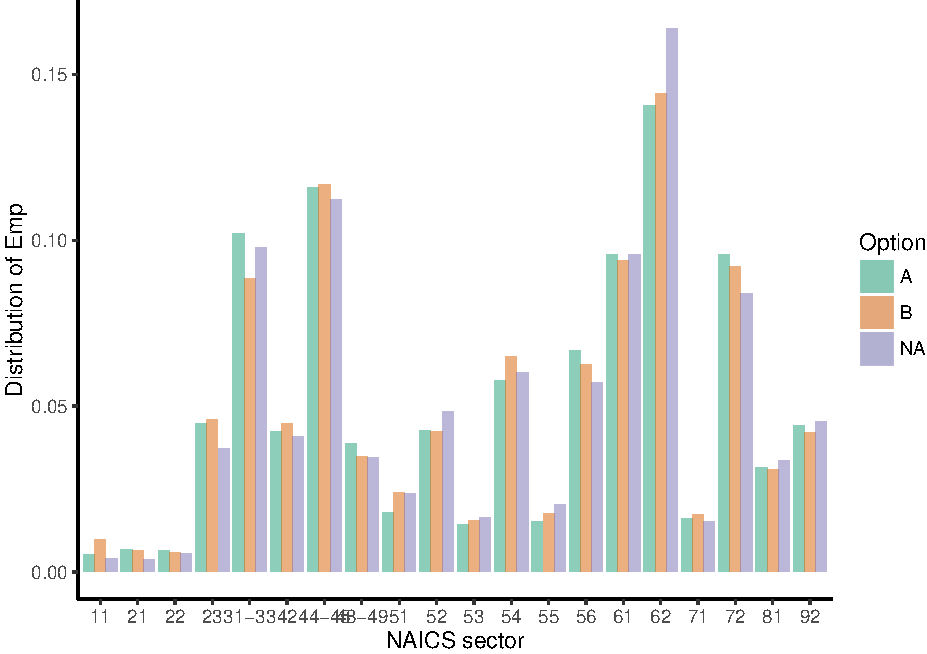
\includegraphics{s2014_availability_files/figure-latex/graph_Emp-1.pdf}

\begin{quote}
Users who want to consider different variables might change the
following option:
\end{quote}

For the industry distribution of \textbf{SepBeg}, the distribution looks
like this:
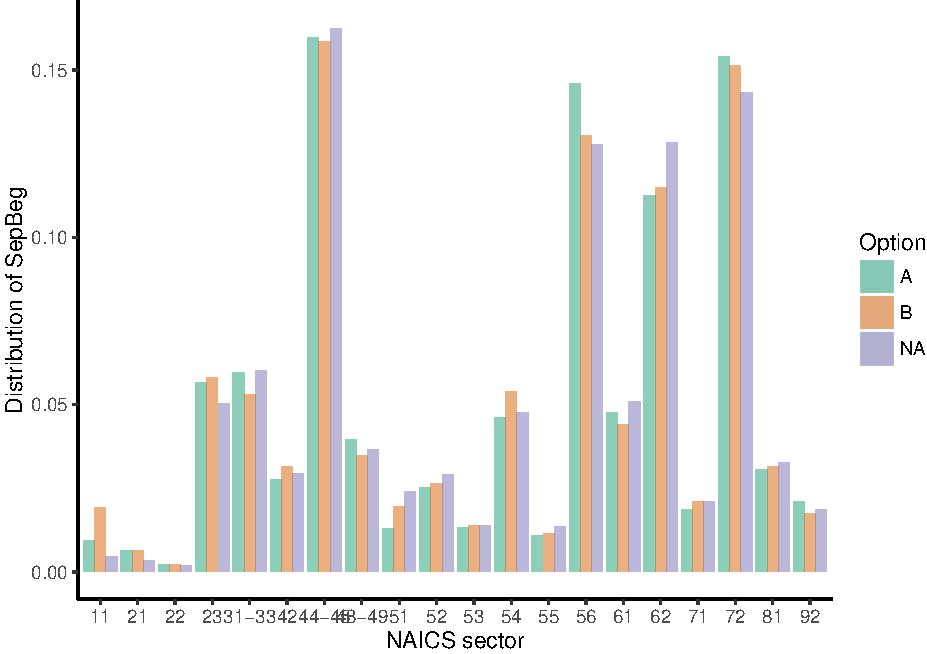
\includegraphics{s2014_availability_files/figure-latex/graph_SepBeg-1.pdf}

For the industry distribution of \textbf{Payroll}, the distribution
looks like this:
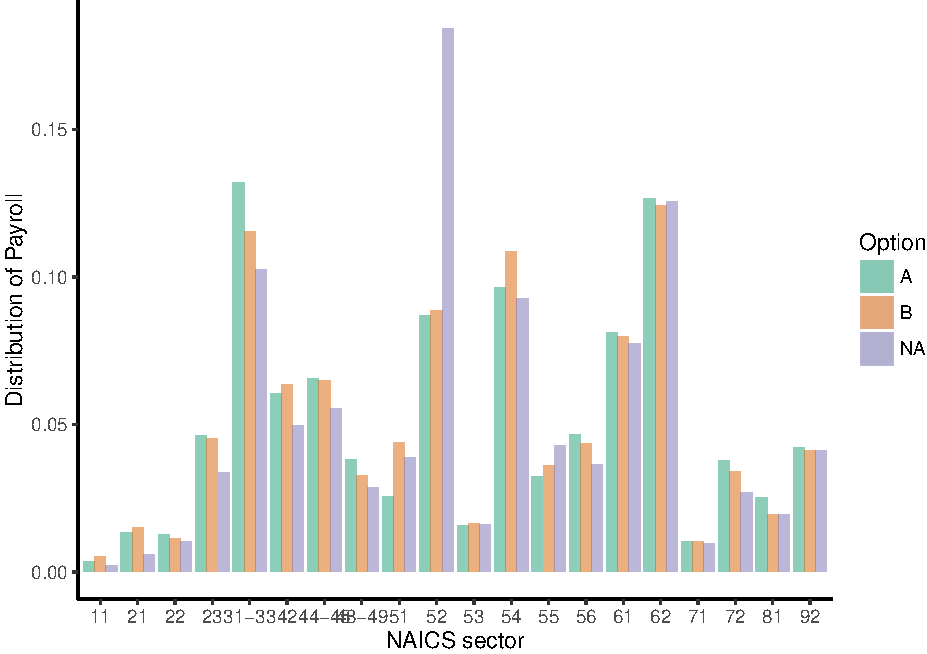
\includegraphics{s2014_availability_files/figure-latex/graph_Payroll-1.pdf}

Additional variables (see the
\href{LEHD\%20Schema}{http://lehd.ces.census.gov/data/schema/V4.0.4/lehd\_public\_use\_schema.html}
for names) can be easily added to the Rmd source file.

\section{Appendix: Full list of state MOUs and option chosen as of
12-10-2015}\label{appendix-full-list-of-state-mous-and-option-chosen-as-of-12-10-2015}

\begin{longtable}[c]{@{}lrlll@{}}
\toprule
& fips & Abbr & Name & Option\tabularnewline
\midrule
\endhead
1 & 1 & AL & Alabama & B\tabularnewline
2 & 2 & AK & Alaska & NA\tabularnewline
3 & 4 & AZ & Arizona & A\tabularnewline
4 & 5 & AR & Arkansas & A\tabularnewline
5 & 6 & CA & California & B\tabularnewline
6 & 8 & CO & Colorado & B\tabularnewline
7 & 9 & CT & Connecticut & B\tabularnewline
8 & 10 & DE & Delaware & A\tabularnewline
9 & 11 & DC & District of Columbia & A\tabularnewline
10 & 12 & FL & Florida & B\tabularnewline
11 & 13 & GA & Georgia & B\tabularnewline
12 & 15 & Hi & Hawaii & B\tabularnewline
13 & 16 & ID & Idaho & B\tabularnewline
14 & 17 & IL & Illinois & A\tabularnewline
15 & 18 & IN & Indiana & A\tabularnewline
16 & 19 & IA & Iowa & A\tabularnewline
17 & 20 & KS & Kansas & A\tabularnewline
18 & 21 & KY & Kentucky & B\tabularnewline
19 & 22 & LA & Louisiana & A\tabularnewline
20 & 23 & ME & Maine & A\tabularnewline
21 & 24 & MD & Maryland & A\tabularnewline
22 & 25 & MA & Massachusetts & B\tabularnewline
23 & 26 & MI & Michigan & NA\tabularnewline
24 & 27 & MN & Minnesota & B\tabularnewline
25 & 28 & MS & Mississippi & NA\tabularnewline
26 & 29 & MO & Missouri & B\tabularnewline
27 & 30 & MT & Montana & B\tabularnewline
28 & 31 & NE & Nebraska & NA\tabularnewline
29 & 32 & NV & Nevada & A\tabularnewline
30 & 33 & NH & New Hampshire & B\tabularnewline
31 & 34 & NJ & New Jersey & B\tabularnewline
32 & 35 & NM & New Mexico & B\tabularnewline
33 & 36 & NY & New York & NA\tabularnewline
34 & 37 & NC & North Carolina & B\tabularnewline
35 & 38 & ND & North Dakota & B\tabularnewline
36 & 39 & OH & Ohio & NA\tabularnewline
37 & 40 & OK & Oklahoma & A\tabularnewline
38 & 41 & OR & Oregon & B\tabularnewline
39 & 42 & PA & Pennsylvania & B\tabularnewline
40 & 44 & RI & Rhode Island & B\tabularnewline
41 & 45 & SC & South Carolina & B\tabularnewline
42 & 46 & SD & South Dakota & NA\tabularnewline
43 & 47 & TN & Tennessee & A\tabularnewline
44 & 48 & TX & Texas & B\tabularnewline
45 & 49 & UT & Utah & B\tabularnewline
46 & 50 & VT & Vermont & B\tabularnewline
47 & 51 & VA & Virginia & B\tabularnewline
48 & 53 & WA & Washington & B\tabularnewline
49 & 54 & WV & West Virginia & B\tabularnewline
50 & 55 & WI & Wisconsin & B\tabularnewline
51 & 56 & WY & Wyoming & NA\tabularnewline
53 & 72 & PR & Puerto Rico & NA\tabularnewline
54 & 78 & VI & Virgin Islands & NA\tabularnewline
\bottomrule
\end{longtable}

\end{document}
